\cotefile{148}
\scanpage{5}
\mspage{1}

\inserted{Exceptional} \uline{curves} \uline{of type} $(1,1)$ (over $\mathbb C$)

A) \uline{Anharmonic} \inserted{elliptic} \uline{curve of square type}

Category of these curves equivalent : that of oriented
\unsure{combinatorial} squares, i.e. of torsors under
\[
\mathbb Z/4\mathbb Z\simeq\mu_4(\mathbb C)\simeq
\begin{gathered}
\text{group of algebraic units}\\
\text{\unsure{in|of} }\mathbb Q[i]
\end{gathered}
\]
\margin{i.e. group of units \unsure{in|of} $\mathbb Z[i]$
(\unsure{ring} of integers of $\mathbb Q[i]$}

The datum of such a torsor \inserted{($S$)} makes it possible to twist
$\mathbb E\ell_0\overset{\mathrm{def}}\simeq\mathbb C/\mathbb Z[i]$
and find
\[
\mathbb E\ell_0(S)\simeq\mathbb E\ell_0
\mathbin{\wedge}_{\mathbb Z/4\mathbb Z}S
\]

\margin{\figure{
% UPPER-DRAWING-BEGIN
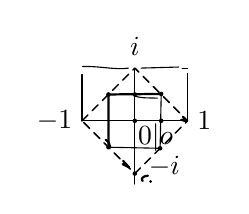
\begin{tikzpicture}[scale=.67,line cap=round,line join=round]
\draw[thin] (-1,0)--(-1,.88);
\draw[thin] (-.99,1.03)..controls(-.65,1.04)and(-.35,.96)..(-.12,1);
\draw[thin] (.12,1)--(.83,1.02);
\draw[thin] (.9,.99)--(1.0,.99);
\draw[thin] (1,.9)--(1,0);
\draw[dash pattern=on 3pt off 2.2pt,line width=.55pt] (-1,0)--(0,1)--(1,0)--(0,-1)--cycle;
\draw (-1,0)--(1,0);
\draw (0,-1.2)--(0,1);
\draw[thick] (-.5,-.5)--(-.5,.5)--(.5,.51);
\draw[thin] (.5,.48)--(.48,-.52)--(-.5,-.5);
\draw[thin] (0,.47)..controls(.15,.42)and(.32,.44)..(.43,.43);
\foreach \x/\y in {0/0,-.5/.5,0/.5,.5/.51,.5/0,.48/-.52,-.5/-.5,0/-1}
{\fill (\x,\y) circle (.043);}
\node[left] at (-1,0) {$-1$};
\node[right] at (1,0) {$1$};
\node[above] at (0,1.06) {$i$};
\node[right] at (.08,-.86) {$-i$};
\node[below right,inner sep=1pt] at (0,0) {$\unsure{0|o}$};
\draw[thick] (.25,-1.04)..controls(.12,-1.05)and(.12,-1.12)..(.15,-1.14);
\fill (.30,-1.15) circle (.028);

\draw[thick] (-.55,-.36)--(-.50,-.40)--(-.47,-.48);
\draw[thick] (.88,.02)--(.98,-.01)--(.91,.08);
\draw[thick] (-.22,-.76)--(-.11,-.88)--(-.23,-.82);
\end{tikzpicture}
% UPPER-DRAWING-END
}}

If the square is realized as a \inserted{Euclidean} square
in a Euclidean plane \inserted{$V_S$} (canonically), with center
$\unsure{0|o}$,
\figure{
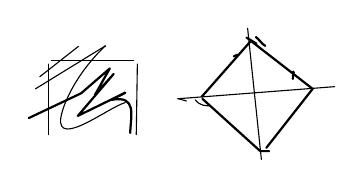
\begin{tikzpicture}[scale=.7,line cap=round,line join=round]
\begin{scope}[xshift=-1.45cm]
% CANCELED-DRAWING-BEGIN
% The cancellation strokes belong to the source drawing.
\draw (-1,-.7)--(-1,.58);
\draw (-.94,.65)--(.55,.65);
\draw (.62,.58)--(.6,-.7);
\draw[thin] (-1.15,.35)--(-.45,.9);
\draw[thin] (-1.23,.13)--(.04,.91);
\draw[thick] (-1.35,-.40)--(-.40,.05)--(.12,.50)--(-.15,.02)--(.19,.40)--(-.46,-.36)--(.40,.06);
\draw[thin] (.04,.91)..controls(-.35,.55)and(-.70,.0)..(-.77,-.40)
..controls(-.84,-.95)and(.12,-.19)..(.40,-.12);
\draw[thick] (.40,.06)--(.15,-.07)..controls(.62,.02)and(.50,-.35)..(.49,-.67);
% CANCELED-DRAWING-END
\end{scope}
\begin{scope}[xshift=1.35cm]
% LIVE-DRAWING-BEGIN
\draw[thick] (-1,0)--(-.12,1.0)--(1,.13)--(.16,-.94);
\draw[thick] (-1,-.05)--(.05,-1.0)--(.21,-1.0);
\draw (-1.45,-.05)--(1.4,.17);
\draw (.07,-1.15)--(-.18,1.23);
\draw[thick] (-.20,1.06)--(-.02,.95);
\draw[thick] (-.03,1.07)..controls(.03,1.03)and(.08,.94)..(.14,.91);
\draw[thick] (-.36,.75)--(-.43,.72);
\draw[thick] (.65,.44)--(.64,.31);
\draw[thin] (-1.13,-.07)..controls(-1.03,-.19)and(-.94,-.17)..(-.85,-.18);
\fill (-1,0) circle (.03);
\fill (.65,.43) circle (.03);
\draw[thin] (-1.43,-.05)--(-1.29,-.09);
% LIVE-DRAWING-END
\end{scope}
\end{tikzpicture}
}
one deduces from it in the plane (a vector space via $\unsure{0|o}$) $V_S$
a system of two \deleted{\unsure{axes} of}
coordinates \inserted{modulo signs,}
via the diagonals, whence a
\deleted{\unsure{lattice|integer}} \inserted{lattice}
\margin{\figure{
% LOWER-DRAWING-BEGIN
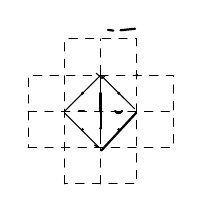
\begin{tikzpicture}[scale=.46,line cap=round,line join=round]
\draw[dashed] (-1,-2)--(-1,2)--(1,2)--(1,-2)--cycle;
\draw[dashed] (-2,-1)--(2,-1)--(2,1)--(-2,1)--cycle;
\draw[dashed] (-2,0)--(2,0);
\draw[dashed] (0,-2)--(0,-1.03);
\draw[dashed] (0,1.04)--(0,2);
\draw[thick] (.20,2.25)--(.35,2.23);
\draw[thick] (.55,2.24)--(.95,2.28);
\draw (-1,0)--(0,1)--(.94,.07);
\draw (-.99,-.05)--(-.04,-1);
\draw[thick] (.98,-.04)--(.02,-1.08);
\draw (0,-.89)--(0,1.14);
\draw[very thick] (0,0)--(0,.50);
\draw[thick] (0,-.47)--(0,0);
\draw[thin] (-.12,1.05)--(.04,.91)--(.12,.98);
\foreach \x/\y in {0/0,-.5/.5,.5/.5,-.5/-.5,.5/-.5,1/1,0/-.47}
{\fill (\x,\y) circle (.045);}

\draw[thick] (-.60,0)--(-.46,0);
\draw[thick] (.40,.01)..controls(.45,-.07)and(.52,-.07)..(.59,.01);
\draw[thin] (-.17,-.93)--(-.08,-.98)--(-.16,-1.00);
\end{tikzpicture}
% LOWER-DRAWING-END
}}
$\Gamma_S$ in $V_S$ (discrete subgroup of
rank $2$) and
\figure{
% ENCLOSURE-BEGIN
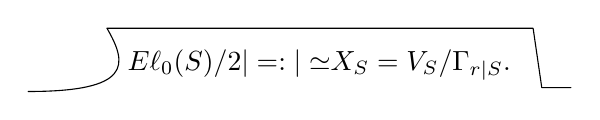
\begin{tikzpicture}[baseline=(F.base),line cap=round,line join=round]
\node[inner sep=3pt] (F) {$\mathbb E\ell_0(\unsure{S})\unsure{/2|=:|\simeq}X_S=V_S/\Gamma_{\unsure{r|S}}.$};
\draw ([xshift=-1.15cm,yshift=-.03cm]F.south west)
..controls([xshift=.16cm,yshift=-.03cm]F.south west)and([xshift=.12cm]F.west)..
([xshift=-.15cm,yshift=.16cm]F.north west)
--([xshift=.17cm,yshift=.16cm]F.north east)
--([xshift=.28cm,yshift=.02cm]F.south east)
--([xshift=.65cm,yshift=.02cm]F.south east);
\end{tikzpicture}
% ENCLOSURE-END
}

There is in $X_S$ a canonical element of order $2$
\inserted{$\eta_S$}
(stable under automorphisms), the other two elements of
order $2$ are interchanged by the generator $i$ of
$\mu_4(\mathbb C)\simeq\operatorname{Aut}(\unsure{X_S})$.
(\uline{NB} $\eta_S$ can therefore be defined

\margin{4}
